%%%%%%%%%%%%%%%% Preamble begins %%%%%%%%%%%%%%%%
\documentclass{article}
\usepackage[utf8]{inputenc}
\usepackage{graphicx} % needed for figures
\usepackage{amsmath} % needed to type beautiful math
\bibliographystyle{elsarticle-num} % a type of bibliography format

%% Some customization here
% needed to have subcaptions with letters in figures
\usepackage{subfig}
\usepackage{subfloat}
\renewcommand*\thesubfloatfigure{\themainfigure(\alph{subfloatfigure})}
\graphicspath{{figures/}}
\captionsetup[subfigure]{subrefformat=simple,labelformat=simple,listofformat=subsimple}
\renewcommand\thesubfigure{(\alph{subfigure})}
%% end of customization

\usepackage{hyperref} % needed to insert hyperref (internal to document) and hyperlinks (urls)
\hypersetup{colorlinks=true,citecolor=blue,linkcolor=blue} % for rendering hyperref and hyperlinks in blue so that they stand out more

\urlstyle{same}

\title{Postdoc Tutorial: Intro on \LaTeX}
\author{Valeria Barra}
\date{\today}

%%%%%%%%%%%%%%%% Preamble ends %%%%%%%%%%%%%%%%%%%%%

%---------------------------------------------%

%%%%%%%%%%%% Actual document body begins %%%%%%%%%%%%

%% Begin document
\begin{document}

\maketitle

\tableofcontents

% similarly, you can create:
\listoffigures
 
\listoftables

% this command pushes the next content on the next page
\clearpage
% Note: In two-sided printing, \cleardoublepage also makes the next page of content a right-hand page, an odd-numbered page, if necessary inserting a blank page

%% Introduction
\section[Intro]{Introduction}
% compare to:
%\section*[Intro]{Introduction} % this prevents this section from being listed and enumerated in the table of contents

This is an introduction to \LaTeX!

But what is \LaTeX? And what is \TeX?

I like this answer from \url{https://tex.stackexchange.com/questions/49/what-is-the-difference-between-tex-and-latex}:

\vspace{\baselineskip} % this inserts a blank line for separation of paragraphs

\noindent ``In short \TeX is all about formatting, for document/template designers, while \LaTeX is all about content, for document writers.

\noindent \TeX is a typesetting system. It provides many commands which allow you to specify the format of your document with great detail (e.g. font styles, spacing, kerning, ligatures, etc.), and has specialized algorithms to compute the optimal flow of text in your document (e.g. where to cut lines, pages, etc.). \TeX is all about giving you powerful algorithms and commands to specify even the tiniest detail to make your documents look pretty.

\noindent \LaTeX is a set of macros built on top of \TeX. The idea behind \LaTeX is to shift the focus from the format to the content of your document. In LaTeX commands are all about giving a structure to the content of your document (e.g. sections, emphasis, tables, indices, etc.). In \LaTeX you just say \texttt{\textbackslash section[...]\{...\}} instead of: selecting a larger font, a different font style, and inserting appropriate spaces before and after the section heading. As LaTeX is built on top of TeX you also get, of course, a beautiful document as your output; but, more importantly, your source input can also be well structured, easier to read (and \emph{write}!) for humans.''

\vspace{\baselineskip} % this inserts a blank line for separation of paragraphs

One of my favorite references from undergrad is \cite{NotSoShortIntro}.

%% Section 2 (the first one is the Introduction, if we haven't used the "*")
\section[Section short title]{Section long title}

This is the first section of our document.

\subsection[Subsec. short title]{Subsection long title}\label{MySection}

I think we need a subsection.

\subsubsection[Subsubsec. short title]{Subsubsection long title}\label{MySubsubsection}

I think we need a subsubsection.

%% Section 3
\section[Section short title]{Section long title}

Now let's start another section. Let's reference something that I said in section \ref{MySection} and elaborated in section \ref{MySubsubsection}.

% an empty line creates a newline
Let's start a new line. % this gets automatically indented

% what if I want a new paragraph not to be indented?
% \noindent forces no indentation
\noindent Let's start a new line that is not automatically indented.

Let's add some vertical spacing.

\texttt{\textbackslash vspace\{\textbackslash baselineskip\}} inserts a blank line, i.e.,~allows you to skip a line with line-spacing given by your current font size.

\vspace{\baselineskip} % this inserts a blank line for separation of paragraphs

first line \smallskip,

second line \medskip, 

third line \bigskip or

a fixed vertical spacing \vspace{1cm}

of $1$~cm. % Note: our first math-mode so far. We include inline math-mode in single $ symbols. The number displayed in math-mode is aesthetically better than in non-math-mode

\vspace{0.5cm}

There are several units in \LaTeX to express spacing. Let's check this \href{https://www.overleaf.com/learn/latex/Lengths_in_LaTeX}{link}.

\vspace{\baselineskip}

Let's look at horizontal spacing. In normal text mode, you can use \mbox{\textbackslash hspace\{ \dots \}} with any desired length. 

In math mode:

\quad	space equal to the current font size (= 18 mu)

\textbackslash,	3/18 of \quad (= 3 mu)

\textbackslash:	4/18 of \quad (= 4 mu)

\textbackslash;	5/18 of \quad (= 5 mu)

\textbackslash!	-3/18 of \quad (= -3 mu)

``\textbackslash \,'' (space after backslash)	equivalent of space in normal text

\textbackslash qquad	twice of \textbackslash quad (= 36 mu)

\vspace{\baselineskip}

Example:

\begin{align}\label{SpacingExample}
f(x) =& x^2\! +3x\! +2 \\
f(x) =& x^2+3x+2 \\
f(x) =& x^2\, +3x\, +2 \\
f(x) =& x^2\: +3x\: +2 \\
f(x) =& x^2\; +3x\; +2 \\
f(x) =& x^2\ +3x\ +2 \\
f(x) =& x^2\quad +3x\quad +2 \\
f(x) =& x^2\qquad +3x\qquad +2
\end{align}



\clearpage % forces the print of all floats (figures and tables) that could not fit and starts the next paragraph in a new page 

% a similar command, \cleardoublepage forces all the floats (tables and images) to be printed and, in a two-sided document always starts the next page on the odd page

%% Section 4
\section[Another section short title]{Another section long title}

% let's create a boring table
% the table environment is needed if you want to caption and reference the table later
\begin{table}[t] % [t] places it at top of page
\begin{tabular}{ l c r }
  1 & 2 & 3 \\
  4 & 5 & 6 \\
  7 & 8 & 9 \\
\end{tabular}
\caption{A very boring table of numbers, not centered in the page.}
\end{table}

\begin{table}[t] % [t] places it at top of page
\centering % this centers everything within this environment
\begin{tabular}{ l | c | r }
  1 & 2 & 3 \\
  4 & 5 & 6 \\
  7 & 8 & 9 \\
\end{tabular}
\caption{A very boring table of numbers, with column separators and centered in the page.}
\end{table}

\begin{table}[ht] % [h] places it here, [ht] is here-top, a bit more elegant
% when LaTeX is stubborn, try "h!" for "really here!" 
\centering % this centers everything within this environment
\begin{tabular}{ |l | c | r| }
  \hline			
  1 & 2 & 3 \\
  4 & 5 & 6 \\
  7 & 8 & 9 \\
  \hline  
\end{tabular}
\caption{A very boring table of numbers, with column and row separators and centered in the page.}
\end{table}

\begin{table}[ht] % [h] places it here, [ht] is here-top, a bit more elegant
% when LaTeX is stubborn, try "h!" for "really here!" 
\centering % this centers everything within this environment
\begin{tabular}{|r|l|}
  \hline
  7C0 & hexadecimal \\
  3700 & octal \\ \cline{2-2} % \cline{i-j}	partial horizontal line beginning in column i and ending in column j
  11111000000 & binary \\
  \hline \hline
  1984 & decimal \\
  \hline
\end{tabular}
\caption{A more complicated table.}
\end{table}

% a more advanced table
\begin{table}[ht] % [h] places it here, [ht] is here-top, a bit more elegant
% when LaTeX is stubborn, try "h!" for "really here!" 
    \centering
    \begin{tabular}{|c|c|c|c|c|c|}
    \hline
    \multicolumn{3}{|c|}{Table of values of $k_{max}$} & \multicolumn{3}{|c|}{Table of values of $\omega_{1_{max}}$} \\ \hline
    $h_0$    & $h_{\star}$ 0.01 & $h_{\star}$ 0.001 & $h_0$    & $h_{\star}$ 0.01 & $h_{\star}$ 0.001 \\ \hline
    1     & 8.3850E-02 & 2.6700E-02 & 1     & 1.0317E-05 & 1.0602E-07 \\ \hline
    0.5   & 2.3550E-01 & 7.5450E-02 & 0.5   & 1.2807E-04 & 1.3529E-06 \\ \hline
    \end{tabular}
    \caption{A more advanced table with multi-columns.}
  \label{tab:ABoringTable}
\end{table}

\clearpage %gets rid of all floating objects (i.e., previous tables in this case) and starts the following text in a new page
Let's add some figures!

\vspace{3em}


\includegraphics[width=0.49\linewidth]{Images/CUBoulderLogo.png}

\vspace{3em}

The top figure is a figure without a \texttt{figure} environment, so it doesn't have a label (i.e., I cannot reference it later) and a caption.


\begin{figure}[h!]
    \centering
    
\includegraphics[width=0.49\linewidth]{Images/CUBoulderLogo.png}
    \caption{This now can be referenced, and it has a very nice caption.}
    \label{fig:CuLogo}
\end{figure}

Let's add two figures side by side:
\begin{figure}[h!]
    \centering
    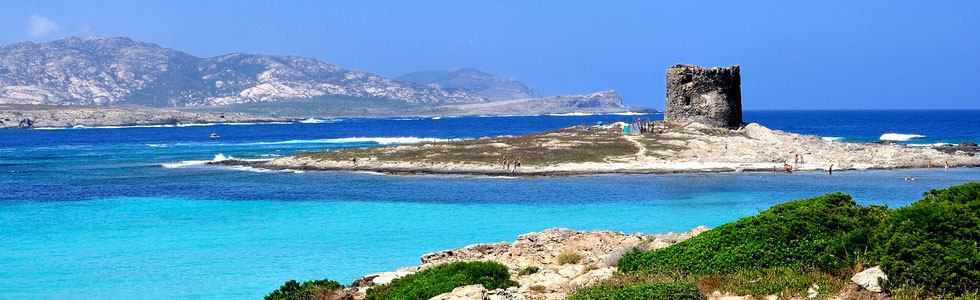
\includegraphics[width=0.5\linewidth]{Images/Stintino.jpg}
    \hspace{2em} % some space in between
    
\includegraphics[width=0.4\linewidth]{Images/Minion.jpg}
    \caption{Sardinia, Italy on the left; a minion on the right.}
    \label{fig:SardiniaAndMinion}
\end{figure}

Now let's add two figures side by side, but in which I can use a subcaption (so I do not need to specify left/right in the caption). For this command I need a bit of work in the preamble.

\begin{figure}
%\captionsetup{type=figure}
    \centering
    \subfloat[]{
\includegraphics[width=0.35\linewidth]{Images//Minion.jpg}\label{fig:Minion}}
    \hfill % it separates the two objects, spanning the entire line
    \subfloat[]{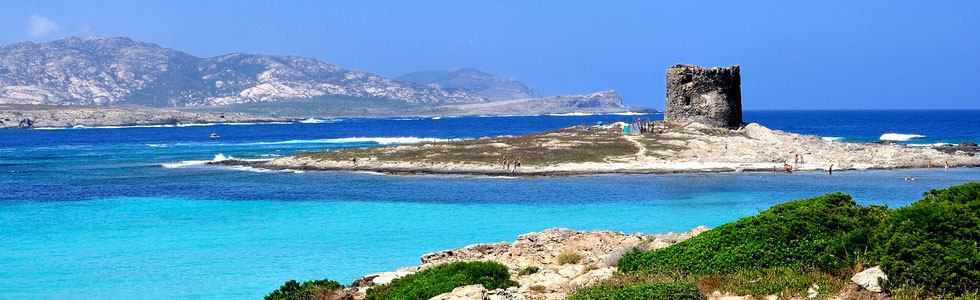
\includegraphics[width=0.5\linewidth]{Images/Stintino.jpg}\label{fig:Stintino}}
    \caption{In \protect\subref{fig:Minion}, a Minion. In \protect\subref{fig:Stintino}, Sardinia, Italy.}
\end{figure}

\clearpage

%% Bibliography
\bibliography{References}



\end{document}
%%%%%%%%%%%% Actual document ends %%%%%%%%%%%%
